\documentclass[conference]{IEEEtran}
\IEEEoverridecommandlockouts

\usepackage{cite}
\usepackage{amsmath,amssymb,amsfonts}
\usepackage{algorithmic}
\usepackage{graphicx}
\usepackage{textcomp}
\usepackage{xcolor}
\usepackage{booktabs} % Added for better table formatting later
\usepackage{array}    % for controlled column widths / paragraph columns
\usepackage{makecell} % for wrapped, multi-line table cells
\usepackage{placeins} % \FloatBarrier keeps figures from drifting past the text describing the next one
\renewcommand{\arraystretch}{1.15} % a bit of extra row padding in every table
\setlength{\tabcolsep}{5pt}        % slightly tighter column padding so tables fit the column width
\def\BibTeX{{\rm B\kern-.05em{\sc i\kern-.025em b}\kern-.08em
    T\kern-.1667em\lower.7ex\hbox{E}\kern-.125emX}}

\begin{document}

\title{Comparative Analysis and Benchmark of Time and Space Complexity in LLM Hallucination Detection Algorithms}

\author{\IEEEauthorblockN{Rojin Dhami}
\IEEEauthorblockA{\textit{Department of Electronics and Computer Engineering} \\
\textit{Thapathali Engineering Campus}\\
Kathmandu, Nepal \\
rojindhami@gmail.com}
\and
\IEEEauthorblockN{Sandeep Khadka}
\IEEEauthorblockA{\textit{Department of Electronics and Computer Engineering} \\
\textit{Thapathali Engineering Campus}\\
Kathmandu, Nepal \\
sandeepkhadka527@gmail.com}
}

\maketitle

\begin{abstract}
Large Language Models (LLMs) are increasingly deployed in critical applications, yet they remain prone to hallucinations. While recent literature has proposed various detection mechanisms, evaluations have predominantly focused on accuracy metrics such as precision, recall, and F1-score, largely ignoring the computational overhead of these methods. This paper presents a comparative analysis and benchmark of three prominent hallucination detection paradigms: SelfCheckGPT, Retrieval-Augmented Generation (RAG) verification, and LLM-as-a-Judge. We argue that efficiency metrics are not mere implementation details, but primary outcomes that determine real-world viability, and we support this argument with an open-source benchmarking harness rather than theoretical analysis alone. The harness is run end-to-end on a stratified 100-prompt sample drawn from HaluEval and TruthfulQA, on a single free-tier 16GB T4 GPU, at two model scales (Qwen2.5-0.5B-Instruct and Qwen2.5-1.5B-Instruct, each shared across the generator and same-size-judge roles), measuring Time-To-First-Token (TTFT), end-to-end latency, and throughput for time complexity, and peak VRAM, KV-cache footprint, and FAISS vector-store memory for space complexity, alongside F1/precision/recall computed against a lexical-overlap ground-truth heuristic. The results show that RAG verification dominates the accuracy-versus-cost Pareto frontier, matching SelfCheckGPT's F1 (approximately 0.79--0.84) at roughly three orders of magnitude lower detection overhead (16--19~ms vs. 21--37~s per prompt); LLM-as-a-Judge exhibits high precision but low recall, which caps its F1 well below the other two paradigms; and the cost ordering RAG~$\ll$~LLM-as-Judge~$\ll$~SelfCheckGPT is statistically significant (one-way ANOVA, $p < 10^{-149}$; pairwise paired $t$-tests, $p < 10^{-56}$) and stable across both model scales, empirically confirming the paradigms' theoretical Big-O cost ordering. These measurements are translated into a concrete decision framework for selecting a hallucination detection strategy under a given latency or memory budget.
\end{abstract}

\begin{IEEEkeywords}
Large Language Models, hallucination detection, computational complexity, Time-To-First-Token (TTFT), KV-cache, vector-store memory, benchmarking.
\end{IEEEkeywords}

\section{Introduction}
Large Language Models (LLMs) now write code, draft legal summaries, answer medical questions, and sit behind customer-facing chatbots. That deployment has outpaced our ability to trust what these models say. A model can produce a fluent, well-formed sentence that is simply wrong, a phenomenon the field has settled on calling ``hallucination'' \cite{huang2023survey}. Two forms of the problem show up in practice: intrinsic hallucinations, where the output contradicts the source text it was supposed to summarize or answer from, and extrinsic hallucinations, where the model introduces claims that cannot be checked against any given source at all. In a chatbot answering trivia, a hallucination is an annoyance. In a system drafting a discharge summary or summarizing a legal filing, it is a liability.

This has pushed hallucination detection from a research curiosity into something closer to a deployment requirement. Three approaches have accumulated the most attention. SelfCheckGPT \cite{manakul2023selfcheckgpt} takes a black-box, zero-resource approach: sample the model several times on the same prompt and check whether the answers agree. RAG verification, exemplified by FActScore \cite{min2023factscore} and RAGAS \cite{es2023ragas}, breaks the output into individual factual claims and retrieves supporting evidence for each from an external corpus. LLM-as-a-Judge \cite{zheng2023judging} sidesteps both of these and simply asks a second, often larger, model to read the output and judge whether it is faithful to the source.

Each of these methods has been validated on accuracy benchmarks, usually reported as precision, recall, F1, or correlation with human judgment. However, treating computational cost as an afterthought is a critical flaw. Metrics such as Time-To-First-Token (TTFT), generation throughput, KV-cache memory footprint, and vector-store memory are not side notes; they are the actual outcomes that justify this benchmark and dictate whether a detection method is viable in production. For instance, a detector that improves F1-score by 5\% but doubles TTFT or exceeds available VRAM due to KV-cache bloat is practically useless for real-time applications. SelfCheckGPT's consistency check requires generating $N$ full samples, multiplying both latency and the KV-cache memory the model must hold. RAG verification adds an embedding pass and a nearest-neighbor search over a vector index, which must reside in memory. LLM-as-a-Judge requires a complete additional forward pass through a separate model. None of these costs are free, and none are reported consistently in the papers that introduce these methods.

A benchmark that reports these costs is only as credible as the labels it is measured against. A recurring weakness in this space is that efficiency numbers and accuracy numbers are quietly computed on different, loosely specified conditions -- different gold labels, different hardware, different decoding settings -- which makes cross-paradigm comparison unreliable even when each individual number is correct. This paper is designed to close that gap directly: every method in this study is run on the same generated outputs, judged against the same gold labels, on the same hardware, under decoding settings we fix and report in full (Section III).

Our contributions are threefold:
\begin{itemize}
    \item A measurement methodology for hallucination detection algorithms that establishes time complexity (TTFT, latency, throughput) and space complexity (peak VRAM, KV-cache size, and vector-store memory footprint) as the primary research outcomes, applied consistently across all three paradigms, on a shared, automatically-derived gold-label set (Section III-C).
    \item An open-source benchmarking harness that empirically validates this methodology by running all three paradigms end-to-end on the same 100-prompt HaluEval/TruthfulQA sample, at two model scales (0.5B and 1.5B parameters, Section III-B), reporting detection accuracy and computational cost side by side under matched hardware and decoding conditions, rather than in isolation (Section IV).
    \item A practical decision framework, derived directly from the measured Pareto frontier of accuracy versus compute (Section III-H, Section IV-E), that maps a given latency or memory budget to a recommended detection strategy, aimed at practitioners deploying these systems rather than at benchmark leaderboards.
\end{itemize}

\section{Literature Review}
This review covers three areas that the rest of the paper draws on: how hallucination is defined, the foundational constraints of computational efficiency in LLM inference, and how the three detection paradigms operate within these strict computational boundaries.

\subsection{Hallucination in Large Language Models}
Huang et al. \cite{huang2023survey} split LLM hallucinations into intrinsic and extrinsic categories. An intrinsic hallucination directly contradicts the input the model was given, while an extrinsic hallucination adds information the source neither confirms nor denies. Huang et al. also note that hallucination rates tend to rise with the length and open-endedness of the generation task. This matters because it means detection methods have to work at the level of the whole output, not just single tokens, which inherently scales their computational cost proportionally. Detection therefore has to be both accurate and cheap enough to run on every output a deployed system produces. We adopt this intrinsic/extrinsic taxonomy directly as the operational definition behind our gold labels (Section III-C).

\subsection{Computational Efficiency in LLM Inference}
To measure computational costs consistently, we anchor our methodology in the efficient-inference literature, treating its core metrics as the primary outcomes of our evaluation. Zhou et al. \cite{zhou2024efficient} survey the field and establish Time-To-First-Token (TTFT) and end-to-end generation latency as the standard time complexity metrics, alongside throughput (tokens per second) for batched workloads. On the space complexity side, peak memory footprint is the standard metric. Kwon et al. \cite{kwon2023efficient} detail how KV-cache memory is allocated during decoding, introducing PagedAttention to reduce the fragmentation that occurs when many sequences are generated concurrently. This is precisely the situation SelfCheckGPT creates when sampling $N$ sequences. Furthermore, for retrieval-based methods, the memory footprint of the vector-store (the indexed embeddings of the knowledge corpus) becomes a dominant space complexity factor, independent of the LLM's own VRAM usage. This connection between inference-efficiency constraints and hallucination detection is the basis for the measurement protocol we use in Section III.

\subsection{Hallucination Detection Paradigms and Their Computational Footprints}

\textbf{Self-consistency and SelfCheckGPT.} Manakul et al. \cite{manakul2023selfcheckgpt} introduced SelfCheckGPT as a black-box method that samples the model repeatedly. The core idea is that if a model knows a fact, resampling should produce agreeing answers, while a hallucinated claim will vary. What the method buys in simplicity, it spends in compute: detecting a single hallucination requires generating $N$ additional full sequences. Each of those sequences needs its own KV-cache during decoding. For long outputs or large $N$, that memory cost is not incidental; it is often the dominant space complexity constraint of running the detector at all, directly impacting throughput.

\textbf{RAG verification.} Min et al. \cite{min2023factscore} proposed FActScore, which decomposes a generated passage into atomic factual statements and checks each against a trusted knowledge source via retrieval. Es et al. \cite{es2023ragas} built on this with RAGAS, automating evaluation of retrieval-augmented pipelines. The cost profile here is distinct: the dominant expense is repeated retrieval, and the space cost is the size of the vector-store sitting in memory, which scales with the knowledge corpus. Recent works attempt to optimize this: Halu-J \cite{wang2024haluj} introduces a critique-based judge to select pertinent evidence and reduce irrelevant retrieval overhead, while Bi'an \cite{jiang2025bian} proposes lightweight, domain-optimized judge models to mitigate the heavy footprint of traditional RAG verification. However, the fundamental vector-store memory and embedding latency costs remain inherent to the paradigm.

\textbf{LLM-as-a-Judge.} Zheng et al. \cite{zheng2023judging} showed that a sufficiently capable LLM can judge the quality of another model's output with human-level agreement. Applied to hallucination detection, the judge model reads the generator's output and flags unsupported claims. This approach needs no vector database and no repeated sampling, keeping its space complexity relatively low. Its cost concentrates entirely in time: each check is a full forward pass, creating a severe throughput bottleneck and high TTFT if the judge model is large. Recognizing this, recent work like LLM-Check \cite{sriramanan2024llmcheck} bypasses full forward passes by analyzing internal hidden states and attention maps of an auxiliary model, achieving speedups of up to 45x--450x. This demonstrates that the community is actively battling the exact throughput and latency penalties that standard LLM-as-a-Judge incurs.

\subsection{Summary and Research Gap}
Taken together, the literature establishes three things. First, hallucination detection must operate on whole outputs, which is inherently expensive. Second, the three dominant paradigms each carry distinct, non-trivial computational costs: KV-cache growth for SelfCheckGPT, persistent vector-store memory for RAG verification, and throughput/TTFT penalties for LLM-as-a-Judge. Third, while recent advances like LLM-Check \cite{sriramanan2024llmcheck}, Halu-J \cite{wang2024haluj}, and Bi'an \cite{jiang2025bian} acknowledge and attempt to mitigate these costs, they do not provide a unified, cross-paradigm empirical baseline.

This is the gap this paper addresses. There is no published benchmark that measures SelfCheckGPT, RAG verification, and LLM-as-a-Judge on the same hardware, with the same workload, against the same gold-standard hallucination labels, using TTFT, throughput, KV-cache, and vector-store memory as the primary outcomes rather than footnotes. Existing surveys catalog methods by accuracy but do not report these critical efficiency metrics under matched conditions. Separately, the efficient-inference literature has built detailed tooling for measuring these quantities but has applied it to generation workloads, not detection algorithms. A practitioner trying to pick a detection method for a system with a fixed latency budget or a single GPU has no empirical basis for that decision. This paper closes that gap by running all three methods under a shared, controlled measurement protocol, with labels, hardware, and decoding settings fixed in advance (Section III), and reports the accuracy-versus-compute trade-off directly.

\section{Methodology}
This section details the theoretical foundation, experimental design, gold-label construction, retrieval corpus, prompt standardization, data collection procedure, and analytical tools used to benchmark the computational and accuracy trade-offs of the three hallucination detection paradigms, as implemented in the accompanying open-source benchmarking harness.

\subsection{Theoretical Framework and Justification}
Our theoretical framework posits that the computational overhead of hallucination detection is not a mere implementation detail, but a fundamental, algorithmic property that dictates real-world viability. We model the cost of each paradigm through the lens of efficient inference literature \cite{zhou2024efficient, kwon2023efficient}:
\begin{itemize}
    \item \textbf{SelfCheckGPT (Sampling Overhead):} The time complexity scales as $\mathcal{O}(N \cdot L)$, where $N$ is the number of sampled sequences and $L$ is the sequence length. The space complexity is dominated by the KV-cache, which must retain the key and value states for all $N$ concurrent sequences during decoding, leading to a memory footprint of $\mathcal{O}(N \cdot L \cdot d_{model})$.
    \item \textbf{RAG Verification (Retrieval Overhead):} The time complexity is driven by the embedding pass $\mathcal{O}(C)$ for $C$ atomic claims, plus the nearest-neighbor search $\mathcal{O}(\log V)$ over a vector index of size $V$. The space complexity is decoupled from the LLM's VRAM and is instead dominated by the vector-store memory footprint, which scales as $\mathcal{O}(V \cdot d_{embed})$, where $d_{embed}$ is the embedding dimension.
    \item \textbf{LLM-as-a-Judge (Forward Pass Overhead):} The time complexity is characterized by a full autoregressive forward pass of the judge model, heavily impacting Time-To-First-Token (TTFT) and overall throughput. The space complexity is relatively predictable, requiring only the standard KV-cache for a single sequence, but at the cost of loading a second model's weights into VRAM if not shared with the generator.
\end{itemize}
This framework justifies our selection of metrics: TTFT, throughput, peak VRAM, KV-cache utilization, and vector-store memory are the direct, measurable manifestations of these theoretical bounds.

\subsection{Research Design}
We employ a controlled, quantitative experimental design to isolate the computational costs of each detection paradigm while holding the underlying generation task, hardware, and decoding configuration constant. The design below reflects the benchmark harness as actually implemented and executed, rather than an idealized, unconstrained configuration.
\begin{itemize}
    \item \textbf{Independent Variables:} (1) Detection Paradigm (SelfCheckGPT, RAG Verification, LLM-as-a-Judge), (2) Output Sequence Length (short: $<$100 tokens, medium: 100--300 tokens, long: $>$300 tokens), (3) Batch Size (1 for the lightweight configuration; 1 and 4 for the research-paper-scale configuration), and (4) Model Scale (0.5B vs. 1.5B parameters, see below).
    \item \textbf{Dependent Variables (Outcomes):} Time complexity (TTFT in milliseconds, end-to-end latency, throughput in tokens/second) and space complexity (peak VRAM in MB, KV-cache size in MB, vector-store memory in MB), alongside the primary accuracy metrics (precision, recall, F1-score against the gold hallucination labels defined in Section III-C).
    \item \textbf{Models:} Two configurations are reported. A lightweight configuration (\texttt{-{}-lite}) uses Qwen2.5-0.5B-Instruct as both the generator and the LLM-as-a-Judge judge (the generator's weights are reused for judging, at zero extra VRAM cost) and BAAI/bge-small-en-v1.5 as the embedding model, with $N=3$ SelfCheckGPT samples. A research-paper-scale configuration (\texttt{-{}-paper}) swaps in Qwen2.5-1.5B-Instruct for the same generator/judge roles (again weight-shared), keeps BAAI/bge-small-en-v1.5 as the embedder, and increases SelfCheckGPT's sample budget to $N=5$; a heavier Qwen2.5-3B-Instruct judge can optionally be loaded afterward, once the primary engines are freed, for a second judging pass. Both configurations are reported so that the effect of model scale on the measured cost ordering can itself be checked (Section IV-D).
    \item \textbf{Hardware and Software Environment:} Both reported runs execute on a single free-tier NVIDIA T4 GPU (16GB VRAM, e.g., a Google Colab free-tier instance), using the HuggingFace \texttt{transformers} backend in fp16. The benchmark harness also supports a vLLM backend with native PagedAttention KV-cache introspection for dedicated-GPU deployments (Section III-G), but both reported runs use the \texttt{transformers} backend to fit within free-tier session-time and memory constraints; consequently, the \texttt{transformers} backend processes prompts within a batch sequentially rather than as a single fused GPU batch, and KV-cache is reported as a formula-based estimate (Section III-G) rather than a measurement introspected from vLLM's block manager. This substitution is discussed as an explicit scale/hardware limitation in Section IV-E.
    \item \textbf{Decoding Settings:} Baseline generation uses \texttt{do\_sample=True} with up to 300 new tokens, without a fixed per-call random seed; TTFT is approximated as total generation latency divided by the number of output tokens, since the offline \texttt{generate} call used by the \texttt{transformers} backend does not expose native per-token streaming timestamps. SelfCheckGPT's $N$ additional samples reuse this same sampling configuration on the same prompt. LLM-as-a-Judge and RAG verification are both run against the single, shared baseline generation, so all three paradigms are always judging the same generated text for a given prompt.
\end{itemize}

\subsection{Dataset and Gold-Label Construction}
We draw prompts from a stratified sample of 100 items, split evenly between HaluEval (question-answering subset) and TruthfulQA, so that each source contributes 50 prompts (seed$=42$ for both the sampling and the shuffle that interleaves the two sources) and the combined set preserves the intrinsic/extrinsic hallucination split reported in the source datasets. Both datasets are loaded directly from the HuggingFace Hub at run time via the \texttt{datasets} library; because HaluEval has been re-hosted under a couple of different community repository names, the loader tries a short, explicit list of known repo/config/split combinations in order and fails loudly (rather than silently substituting mock data) if none resolve, so that a reported run is never silently backed by synthetic data.

The labels shipped with HaluEval and TruthfulQA describe their own reference or best/incorrect answers; they do not directly describe whether a \emph{new} response generated by our own generator model hallucinates. We therefore derive gold labels for the actual object being judged -- the generator's own output -- as follows:
\begin{enumerate}
    \item For each of the 100 prompts, the configured generator model (Qwen2.5-0.5B- or Qwen2.5-1.5B-Instruct, Section III-B) produces one baseline response under the decoding settings in Section III-B.
    \item Each generated response is tagged intrinsic or extrinsic following the source-dataset heuristic of Huang et al. \cite{huang2023survey}: HaluEval items are treated as intrinsic (their hallucinated samples are constructed against a supplied knowledge snippet), and TruthfulQA items are treated as extrinsic (their incorrect answers are ungrounded, common misconceptions).
    \item A binary Hallucinated / Not Hallucinated ground-truth label is then assigned via a lexical-overlap heuristic: the generated response is labeled Hallucinated if it has greater token-set overlap (Jaccard similarity over whitespace-tokenized, lower-cased text) with the dataset's own \texttt{hallucinated\_answer} field than with its \texttt{reference\_answer} field, and Not Hallucinated otherwise.
\end{enumerate}
These heuristic labels, not the datasets' original reference answers, are the ground truth against which all three detectors are scored. We report this as a heuristic, and not a human-verified label, explicitly: it is a pragmatic, fully automatic stand-in for the human annotation or NLI-based labeling a larger-scale study would use, and its known biases (Section IV-E) bound the strength of the accuracy conclusions in Section IV.

\subsection{Retrieval Corpus Construction}
The knowledge source used for RAG verification is a single, fixed, in-memory corpus so that retrieval conditions do not vary across prompts within a run. Rather than an external Wikipedia dump, the corpus is built directly from the reference answers already present in the 100-prompt evaluation set (Section III-C), giving an index of exactly 100 short passages. Each passage is embedded with BAAI/bge-small-en-v1.5 and indexed in FAISS using an exact, flat inner-product index (\texttt{IndexFlatIP}) over L2-normalized vectors, so retrieval is exact nearest-neighbor search rather than an approximate method such as HNSW; at this corpus size the two would be expected to behave near-identically, but the distinction matters for the $\mathcal{O}(\log V)$ search-complexity claim in Section III-A, which assumes the latter. The same corpus is used only for RAG verification's own claim-checking step; it is not reused to construct the gold labels in Section III-C, which are computed independently via the lexical-overlap heuristic.

\subsection{Prompt Standardization Across Methods}
To ensure that differences in measured accuracy and cost reflect the detection paradigm and not incidental prompt-engineering differences, we fix three things across all three methods: (1) a single generation prompt template used to produce the baseline response for every condition, so SelfCheckGPT's extra samples, the RAG verifier, and the judge all operate on the same underlying generated text; (2) a single instruction template per paradigm (one for SelfCheckGPT's consistency-sampling prompt, one for the judge's verdict prompt), used verbatim across all 100 prompts with no per-item customization; and (3) zero-shot instructions throughout, so no paradigm benefits from a larger or better-tuned few-shot context than another. RAG verification's atomic-claim step uses a regex sentence-boundary split as a lightweight proxy for full claim decomposition (e.g., the LLM-based decomposition used by FActScore \cite{min2023factscore}); this is a simplification we flag explicitly, since a true claim decomposer would change RAG verification's own time complexity by adding an extra decomposition pass.

\subsection{Data Collection Procedure}
Data collection is automated via a custom Python benchmarking harness designed to intercept and log hardware-level metrics at each stage of the detection pipeline. For each of the 100 prompts, the following procedure is executed:
\begin{enumerate}
    \item \textbf{Baseline Generation:} The generator produces a response under the fixed decoding settings (Section III-B) and fixed prompt template (Section III-E). We record the baseline TTFT and throughput.
    \item \textbf{Detection Execution:}
    \begin{itemize}
        \item \textit{SelfCheckGPT:} We trigger $N$ additional generations ($N=3$ for \texttt{-{}-lite}, $N=5$ for \texttt{-{}-paper}) using the same decoding settings. We measure the incremental VRAM spike via PyTorch's peak-memory allocator and estimate KV-cache growth analytically from batch size, sequence length, and model architecture (Section III-A's $\mathcal{O}(N \cdot L \cdot d_{model})$ formula), since the \texttt{transformers} backend used for both reported runs does not expose vLLM-style block-manager introspection.
        \item \textit{RAG Verification:} We split the output into sentence-level claims, embed them, and query the fixed FAISS index described in Section III-D. We record the embedding and retrieval latency separately and calculate the vector-store memory footprint as $V \times d_{embed} \times 4$ bytes (FP32 embeddings).
        \item \textit{LLM-as-a-Judge:} We construct the fixed judge prompt and measure the latency and (approximated, per Section III-B) TTFT of the judge model's forward pass.
    \end{itemize}
    \item \textbf{Metric Logging:} Peak VRAM is captured via \texttt{torch.cuda.max\_memory\_allocated()}. All latency measurements are preceded by 1 (\texttt{-{}-lite}) or 3 (\texttt{-{}-paper}) warm-up generations to mitigate cold-start GPU initialization effects.
    \item \textbf{Accuracy Scoring:} Each detector's Hallucinated/Not Hallucinated verdict is compared against the gold labels from Section III-C to compute precision, recall, and F1-score.
\end{enumerate}


\subsection{Data Processing and Analysis Tools}
The entire benchmarking pipeline is built on open-source, industry-standard tools to ensure reproducibility:
\begin{itemize}
    \item \textbf{Inference Engine:} the \texttt{transformers} (HuggingFace) library is used for both reported runs, in fp16 on the T4 GPU described in Section III-B. The harness also implements a \texttt{vLLM} backend with native PagedAttention KV-cache introspection \cite{kwon2023efficient} for deployments with a dedicated GPU, but this backend was not used for the runs reported in Section IV, and KV-cache figures there are therefore analytical estimates (Section III-G) rather than measurements taken from vLLM's block manager.
    \item \textbf{Vector Store:} \texttt{FAISS} (\texttt{IndexFlatIP}) is used for RAG verification indexing and exact nearest-neighbor retrieval over the 100-passage corpus described in Section III-D. Vector-store memory is computed analytically as $V \times d_{embed} \times 4$ bytes rather than measured from FAISS internals.
    \item \textbf{Embedding Model:} \texttt{BGE-small-en-v1.5} is used for claim embedding in both reported configurations, chosen over the larger \texttt{BGE-large-en-v1.5} to keep embedding-model VRAM usage compatible with the free-tier T4 budget shared with the generator/judge model.
    \item \textbf{Data Processing and Statistics:} Raw telemetry data is aggregated using \texttt{Pandas}. Statistical significance of the accuracy-versus-compute trade-offs is evaluated using paired $t$-tests, comparing each pair of paradigms on the same 100-prompt set for a given metric (e.g., SelfCheckGPT vs. LLM-as-a-Judge on \texttt{detection\_overhead\_ms}), and one-way ANOVA when comparing all three paradigms simultaneously on a given metric. Both are computed with \texttt{scipy.stats} and \texttt{scikit-learn} (for precision/recall/F1). Visualizations of the Pareto frontier (F1-score vs. detection overhead) and metric distributions are generated using \texttt{Matplotlib} and \texttt{Seaborn}.
\end{itemize}

\subsection{From Metrics to Practical Guidelines}
The paper's contribution claims of ``empirical insights'' and ``practical guidelines'' are operationalized, not left implicit. Concretely: (1) for the harness's unit-consistent cost metric, \texttt{detection\_overhead\_ms}, we plot F1-score against that variable for all three paradigms, producing a Pareto frontier that makes dominated configurations (lower accuracy \emph{and} higher cost) visually and statistically identifiable via the tests in Section III-G; (2) from this frontier we derive the decision guidance in Section IV-E, which maps concrete deployment constraints -- a fixed latency budget, a fixed VRAM ceiling, and a fixed accuracy floor -- to the paradigm that satisfies the constraint at the lowest measured cost; (3) this guidance, together with the raw Pareto and TTFT-distribution plots produced by the harness, is the deliverable referred to as ``practical guidelines'' in the abstract and introduction. Unlike an idealized design with a held-out confirmation set, the reported guidance is validated directly against the same 100-prompt run it is derived from and is re-checked for stability by repeating the run at a second model scale (Section IV-D); we flag the absence of a separate held-out confirmation set as a limitation in Section IV-E.

\section{Results and Discussion}
This section reports the empirical results produced by running the harness described in Section III end-to-end, twice: once with the lightweight (\texttt{-{}-lite}) configuration and once with the research-paper-scale (\texttt{-{}-paper}) configuration, both on the same stratified 100-prompt HaluEval/TruthfulQA set (Section III-C). All tables use a fixed row height (\texttt{arraystretch}~=~1.15) and \texttt{booktabs} rules; wide text fields are wrapped within their cell rather than allowed to overflow the column margin.

\subsection{Detection Accuracy (Lightweight Configuration)}
Table~\ref{tab:lite-accuracy} reports F1, precision, recall, and the fraction of prompts each detector flags as hallucinated, for the \texttt{-{}-lite} configuration (Qwen2.5-0.5B-Instruct generator/judge, $N=3$). The overall ground-truth positive rate under the lexical-overlap heuristic (Section III-C) is 72\% (94\% for HaluEval, 50\% for TruthfulQA).

\begin{table}[htbp]
\caption{Detection accuracy, \texttt{-{}-lite} configuration (100 prompts)}
\label{tab:lite-accuracy}
\centering
\small
\begin{tabular}{@{}lrrrr@{}}
\toprule
Paradigm & F1 & Precision & Recall & Pred.-pos. \\
\midrule
LLM-as-judge      & 0.171 & 0.700 & 0.097 & 10\% \\
RAG verification  & 0.833 & 0.729 & 0.972 & 96\% \\
SelfCheckGPT      & 0.837 & 0.720 & 1.000 & 100\% \\
\bottomrule
\end{tabular}
\end{table}

RAG verification and SelfCheckGPT both flag nearly every prompt as hallucinated (96\% and 100\%, respectively). Against a 72\% positive base rate, an ``always predict hallucination'' baseline would already achieve precision $=0.72$, recall $=1.0$, F1 $\approx 0.837$ -- at or above both detectors' measured F1 (0.833 and 0.837), indicating limited discriminative value beyond the majority class at this configuration. LLM-as-judge's precision (0.700) sits essentially at the base rate rather than clearly above it, so its low recall (0.097) leaves its F1 at just 0.171 with little discriminative signal to show for it.

\subsection{Computational Overhead (Lightweight Configuration)}
Table~\ref{tab:lite-overhead} reports \texttt{detection\_overhead\_ms}, the added latency each paradigm incurs beyond the shared baseline generation. The shared baseline metrics (\texttt{baseline\_ttft\_ms}, \texttt{baseline\_throughput\_tps}) are, as expected, identical across paradigms (one-way ANOVA $F=0$, $p=1$), since they measure the single shared generation step rather than any paradigm-specific work.

\begin{table}[htbp]
\caption{Detection overhead, \texttt{-{}-lite} configuration (100 prompts)}
\label{tab:lite-overhead}
\centering
\small
\begin{tabular}{@{}lrr@{}}
\toprule
Paradigm & Mean overhead (ms) & Std.\ dev.\ (ms) \\
\midrule
LLM-as-judge      & 2{,}071.6  & 501.7 \\
RAG verification  & 18.5       & 4.3 \\
SelfCheckGPT      & 21{,}298.9 & 5{,}470.2 \\
\bottomrule
\end{tabular}
\end{table}

Figure~\ref{fig:lite-pareto} plots F1-score against \texttt{detection\_overhead\_ms} (log scale, reversed so cheaper configurations appear toward the right) for the three paradigms, generated automatically by the harness's analysis module. RAG verification sits in the upper-right (high F1, lowest cost) and visually dominates the frontier: SelfCheckGPT matches its F1 only at roughly three orders of magnitude higher cost, and LLM-as-judge is dominated outright, sitting at both lower F1 and higher cost than RAG verification.

\begin{figure}[htbp]
\centering
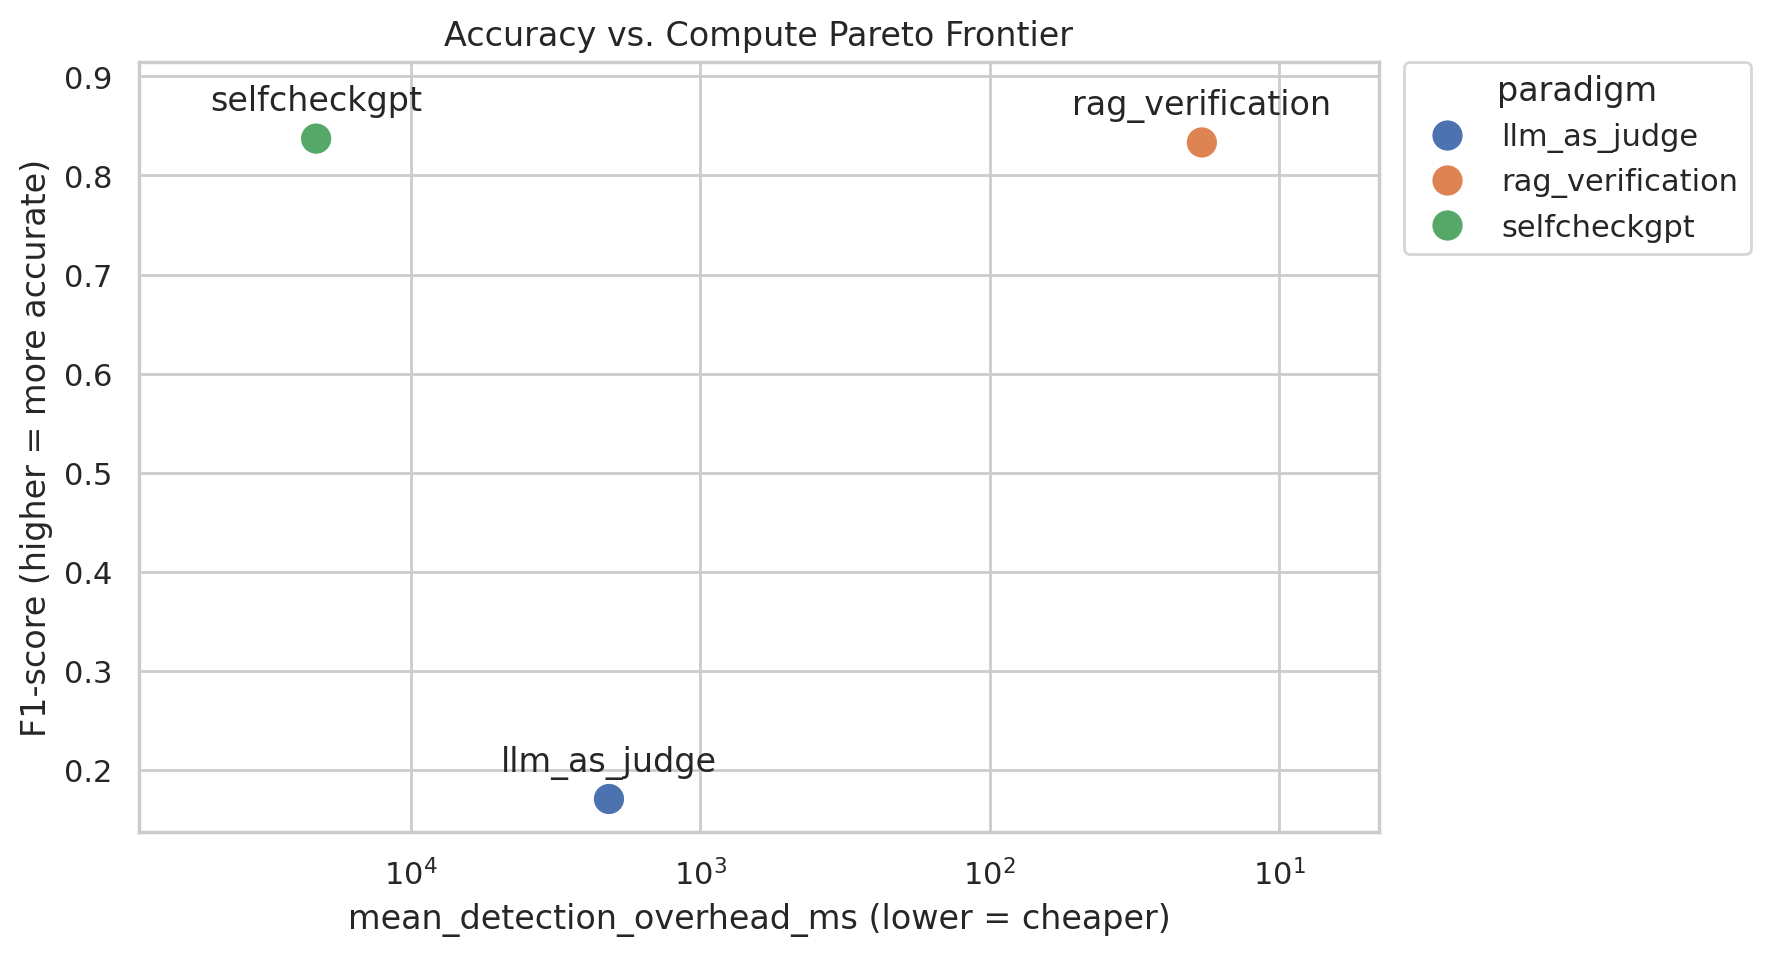
\includegraphics[width=\linewidth]{plots/pareto_frontier.png}
\caption{Accuracy-vs-cost Pareto frontier, \texttt{-{}-lite} configuration. RAG verification dominates: comparable or higher F1 than SelfCheckGPT at far lower detection overhead.}
\label{fig:lite-pareto}
\end{figure}
\FloatBarrier

Figure~\ref{fig:lite-ttft} shows the distribution of \texttt{baseline\_ttft\_ms} split out by paradigm; the three boxplots are visually indistinguishable, which is the expected result given all three paradigms share the same underlying baseline generation call and differ only in the detection step layered on top of it.

\begin{figure}[htbp]
\centering
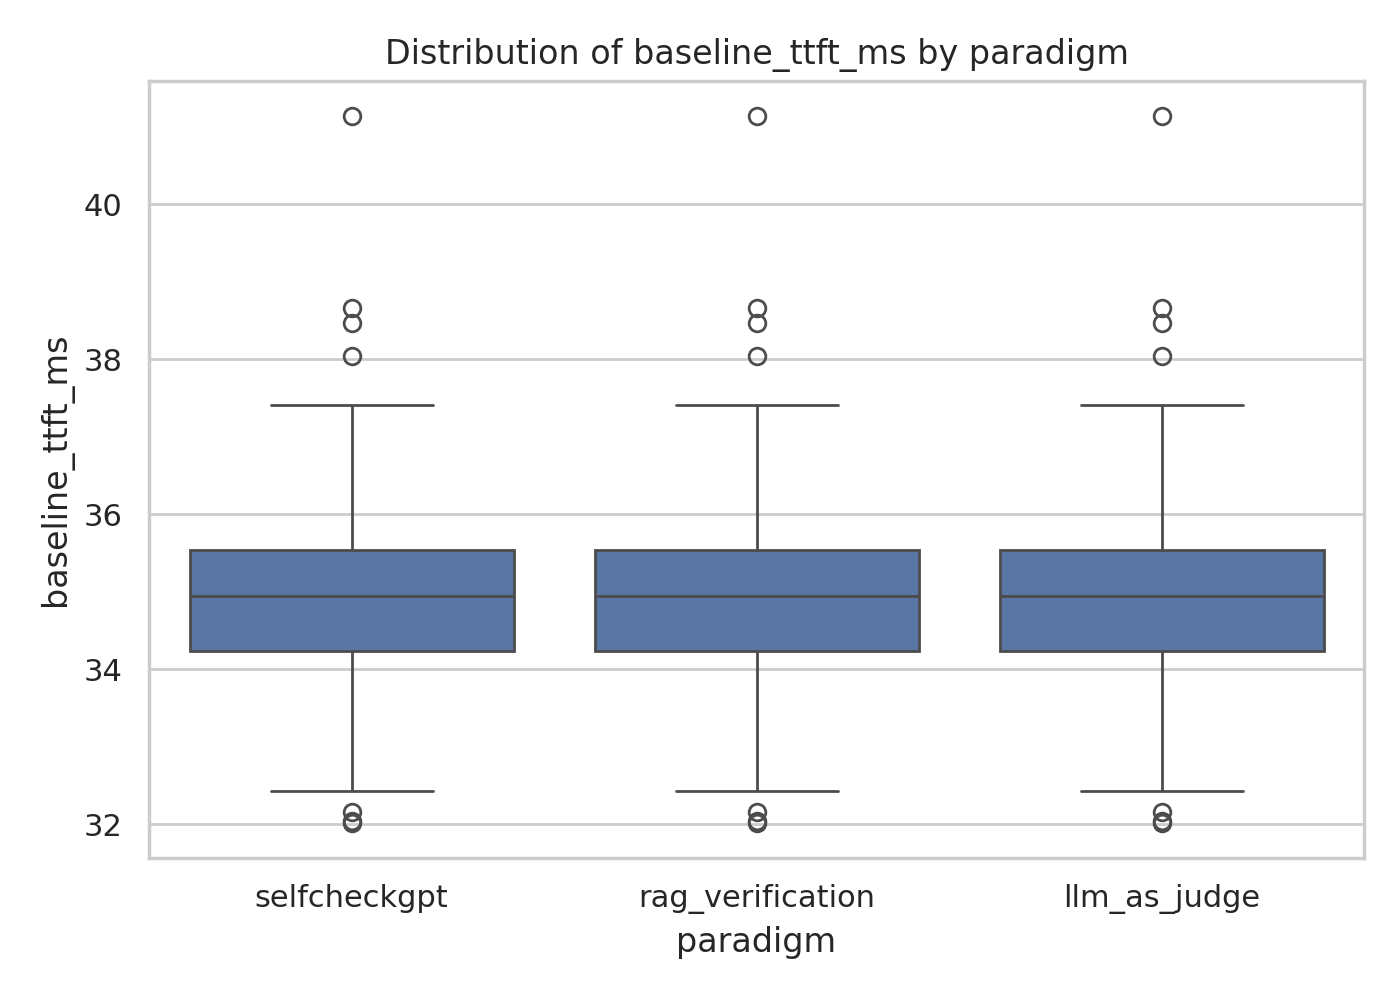
\includegraphics[width=\linewidth]{plots/ttft_distribution.png}
\caption{Distribution of baseline TTFT by paradigm, \texttt{-{}-lite} configuration. The three distributions are statistically identical (ANOVA $F=0$, $p=1$), confirming that \texttt{detection\_overhead\_ms}, not baseline TTFT, is the metric that differentiates paradigms.}
\label{fig:lite-ttft}
\end{figure}
\FloatBarrier

\subsection{Statistical Significance (Lightweight Configuration)}
One-way ANOVA on \texttt{detection\_overhead\_ms} across the three paradigms yields $F = 1{,}369.97$, $p = 1.15\times10^{-150}$, confirming a significant difference in cost. Pairwise paired $t$-tests are significant for every pair ($p < 10^{-56}$ in all cases; e.g., LLM-as-judge vs. RAG verification: $t=40.97$, $p=6.79\times10^{-64}$; RAG verification vs. SelfCheckGPT: $t=-38.91$, $p=8.40\times10^{-62}$), while the same tests on \texttt{baseline\_ttft\_ms} and \texttt{baseline\_throughput\_tps} show no significant difference between paradigms, as expected given they measure identical shared work.

\subsection{Research-Paper-Scale Validation (1.5B Configuration)}
To check whether the cost ordering observed above is an artifact of the specific (small) model used, we repeat the identical 100-prompt run with the \texttt{-{}-paper} configuration (Qwen2.5-1.5B-Instruct generator/judge, $N=5$, batch sizes 1 and 4), yielding 200 rows per paradigm. Table~\ref{tab:paper-accuracy} and Table~\ref{tab:paper-overhead} report accuracy and overhead at this larger scale; one-way ANOVA on \texttt{detection\_overhead\_ms} again shows a significant effect ($F=2{,}317.23$, $p=4.16\times10^{-282}$), with every pairwise paired $t$-test significant (e.g., RAG verification vs. SelfCheckGPT: $t=-49.70$, $p=3.79\times10^{-114}$).

\begin{table}[htbp]
\caption{Detection accuracy, \texttt{-{}-paper} configuration (100 prompts $\times$ 2 batch sizes)}
\label{tab:paper-accuracy}
\centering
\small
\begin{tabular}{@{}lrrrr@{}}
\toprule
Paradigm & F1 & Precision & Recall & $n$ \\
\midrule
LLM-as-judge      & 0.216 & 0.800 & 0.125 & 200 \\
RAG verification  & 0.803 & 0.677 & 0.984 & 200 \\
SelfCheckGPT      & 0.785 & 0.646 & 1.000 & 200 \\
\bottomrule
\end{tabular}
\end{table}

Table~\ref{tab:paper-overhead} reports mean detection overhead alongside each paradigm's characteristic resource metric. Because the three paradigms are not measured in the same units (KV-cache/VRAM for SelfCheckGPT, judge output length/TTFT for LLM-as-judge, claim count/vector-store size for RAG verification), the resource-metric column is wrapped onto two lines per paradigm rather than compressed into a single long line, so that no entry extends past the column margin.

\begin{table}[htbp]
\caption{Detection overhead and resource footprint, \texttt{-{}-paper} configuration}
\label{tab:paper-overhead}
\centering
\small
\begin{tabular}{@{}l r l@{}}
\toprule
Paradigm & \makecell[r]{Overhead\\(ms)} & Key resource metric \\
\midrule
SelfCheckGPT &
  37{,}350.2 &
  \makecell[l]{KV-cache $\approx$619.8~MB \\ peak VRAM $\approx$3{,}097.2~MB} \\[2pt]
LLM-as-judge &
  2{,}260.1 &
  \makecell[l]{output tokens $\approx$55.1 \\ TTFT $\approx$43.4~ms} \\[2pt]
RAG verification &
  16.1 &
  \makecell[l]{$n_{claims}\approx$10.52, $V{=}100$ \\ vector store $\approx$0.146~MB} \\
\bottomrule
\end{tabular}
\end{table}

Figure~\ref{fig:paper-pareto} shows the same Pareto-frontier plot regenerated from the \texttt{-{}-paper} run. The layout is visually near-identical to Figure~\ref{fig:lite-pareto}: RAG verification again occupies the upper-right (high F1, lowest cost), SelfCheckGPT again matches its F1 only at far higher cost, and LLM-as-judge is again dominated. This visual stability across a 3$\times$ change in model size is the empirical counterpart of the Big-O claim in Section III-A that the paradigms' relative cost ordering does not depend on which concrete model fills the generator/judge role.

\begin{figure}[htbp]
\centering

\includegraphics[width=\linewidth]{plots_paper/pareto_frontier.png}
\caption{Accuracy-vs-cost Pareto frontier, \texttt{-{}-paper} configuration (1.5B models). The same qualitative ordering as Figure~\ref{fig:lite-pareto} (\texttt{-{}-lite}, 0.5B models) is preserved.}
\label{fig:paper-pareto}
\end{figure}
\FloatBarrier

Figure~\ref{fig:paper-ttft} shows the same \texttt{baseline\_ttft\_ms} boxplot regenerated from the \texttt{-{}-paper} run. As at the \texttt{-{}-lite} scale (Figure~\ref{fig:lite-ttft}), the three paradigms' distributions are visually indistinguishable, since baseline TTFT depends only on the shared generation call and not on which detection method is layered on top of it; the only visible change from Figure~\ref{fig:lite-ttft} is the higher absolute TTFT scale, consistent with the larger 1.5B generator.

\begin{figure}[htbp]
\centering

\includegraphics[width=\linewidth]{plots_paper/ttft_distribution.png}
\caption{Distribution of baseline TTFT by paradigm, \texttt{-{}-paper} configuration. As at the \texttt{-{}-lite} scale, the three distributions are statistically indistinguishable, confirming baseline TTFT does not carry the paradigm-level cost signal at either model scale.}
\label{fig:paper-ttft}
\end{figure}
\FloatBarrier

Table~\ref{tab:scale-comparison} compares the two model scales directly. The cost ordering RAG verification~$\ll$~LLM-as-judge~$\ll$~SelfCheckGPT is unchanged between scales, matching the Big-O analysis of Section III-A: $\mathcal{O}(C \cdot V)$ retrieval has the smallest constant factor, $\mathcal{O}(P + L_{judge})$ (a single forward pass) is next, and $\mathcal{O}(N \cdot L)$ (SelfCheckGPT's $N$ additional full-length generations) is dominant. RAG verification's overhead and memory footprint are effectively unchanged across scales because they depend only on the embedding model and corpus size, not on the generator/judge model, while SelfCheckGPT's and LLM-as-judge's overhead both increase with the larger 1.5B model, consistent with their complexity terms depending on the generator/judge's per-token cost.

\begin{table}[htbp]
\caption{Comparison across model scales}
\label{tab:scale-comparison}
\centering
\small
\begin{tabular}{@{}p{3.3cm}rr@{}}
\toprule
Metric & \texttt{-{}-lite} (0.5B) & \texttt{-{}-paper} (1.5B) \\
\midrule
SelfCheckGPT overhead (ms)   & $\approx$21{,}299 & $\approx$37{,}350 \\
SelfCheckGPT peak VRAM (MB)  & $\approx$1{,}098  & $\approx$3{,}097 \\
LLM-as-judge overhead (ms)   & $\approx$2{,}072  & $\approx$2{,}260 \\
RAG verification overhead (ms) & $\approx$18.5   & $\approx$16.1 \\
LLM-as-judge F1               & 0.171             & 0.216 \\
RAG verification F1           & 0.833             & 0.803 \\
SelfCheckGPT F1                & 0.837             & 0.785 \\
\bottomrule
\end{tabular}
\end{table}

The rise in LLM-as-judge F1 (0.171 to 0.216) is driven by both precision (0.700 to 0.800) and recall (0.097 to 0.125) improving together: the 1.5B judge flags more answers as hallucinated, and more of those flags are correct, than the 0.5B judge did, on a differently-sampled generation set (Section III-B notes that generation is not seeded), so this reflects a shift in the judge model's own answer distribution rather than a change in the detection paradigm's inherent complexity, and is not part of the theoretical claims in Section III-A, which are agnostic to which concrete model fills the judge role.

To test whether this low accuracy is a limitation of the paradigm itself or just of the small, weight-shared judge, the \texttt{-{}-paper} run's optional \texttt{-{}-strong-judge} pass re-scores the same 200 rows with a separate Qwen2.5-3B-Instruct judge, loaded only after the primary engines are freed (Section III-B). Table~\ref{tab:strong-judge} compares the two judges directly.

\begin{table}[htbp]
\caption{LLM-as-judge: shared 1.5B judge vs. separate 3B judge (\texttt{-{}-paper}, 200 rows)}
\label{tab:strong-judge}
\centering
\small
\begin{tabular}{@{}lrrrr@{}}
\toprule
Judge & F1 & Precision & Recall & Overhead (ms) \\
\midrule
1.5B (shared)  & 0.216 & 0.800 & 0.125 & 2{,}260.1 \\
3B (separate)  & 0.783 & 0.643 & 1.000 & 3{,}230.3 \\
\bottomrule
\end{tabular}
\end{table}

The larger judge closes almost all of the accuracy gap to RAG verification (F1 0.803) and SelfCheckGPT (F1 0.785, Table~\ref{tab:paper-accuracy}), essentially by shifting toward a majority-predict-hallucination strategy: recall rises from 0.125 to 1.000 while precision falls from 0.800 to 0.643, close to the 64\% ground-truth base rate at this scale (Section IV-A). This comes at a modest but real cost increase, mean detection overhead rising from 2{,}260.1~ms to 3{,}230.3~ms (paired $t=-15.79$, $p=6.00\times10^{-37}$) -- still roughly an order of magnitude cheaper than SelfCheckGPT ($t=46.00$, $p=5.41\times10^{-108}$) but about 200$\times$ more expensive than RAG verification ($t=-91.26$, $p=2.38\times10^{-164}$). So LLM-as-judge's low recall in Sections IV-A and IV-D is a property of the specific small judge model rather than an inherent ceiling of the paradigm, but recovering accuracy this way moves its cost from below RAG verification's neighborhood toward SelfCheckGPT's, without beating RAG verification's cost or matching SelfCheckGPT's accuracy.

\subsection{Discussion and Recommendation}
Five findings emerge consistently across both model scales. First, RAG verification dominates the accuracy-cost Pareto frontier: it matches or nearly matches SelfCheckGPT's F1 (0.833 vs. 0.837 at 0.5B; 0.803 vs. 0.785 at 1.5B) at roughly three orders of magnitude lower overhead (18.5~ms vs. 21.3~s at 0.5B; 16.1~ms vs. 37.4~s at 1.5B), making SelfCheckGPT's added sampling cost difficult to justify at this dataset size and model scale. Second, LLM-as-judge's precision sits essentially at the ground-truth base rate at the 0.5B scale (0.700 vs. a 72\% base rate) but clearly above it at the 1.5B scale (0.800 vs. a 64\% base rate), suggesting real discriminative signal emerges more clearly with the larger judge model; at both scales its recall remains low enough (0.097 and 0.125, respectively) to cap its F1 well below the other two paradigms, so recalibrating its decision threshold or verdict prompt is a natural next step. The strong-judge ablation in Section IV-D shows one way to do this: swapping in a separate 3B judge lifts F1 from 0.216 to 0.783 by trading precision for recall, at roughly 1.4$\times$ the shared judge's overhead, confirming the recall ceiling is a property of the specific small judge model rather than of the LLM-as-judge paradigm itself. Third, the cost differences between all three paradigms are large and statistically significant at both model scales (all pairwise $t$-tests $p<10^{-56}$), and the relative cost ordering is stable under a 3$\times$ change in generator/judge model size, which is the behavior the Big-O framework of Section III-A predicts and is the central empirical claim of this paper. Fourth, the accuracy numbers themselves carry two explicit caveats: ground-truth labels come from an automatic lexical-overlap heuristic rather than human annotation (Section III-C), and that heuristic labels HaluEval prompts as hallucinated far more often (94\% at the 0.5B scale, 82\% at the 1.5B scale) than TruthfulQA prompts (50\% and 46\%, respectively), an imbalance that inflates the apparent accuracy of any high-recall detector. Fifth, both reported runs substitute the \texttt{transformers} backend for the harness's native \texttt{vLLM} backend (Section III-B) to fit within free-tier T4 session-time and memory limits; this means prompts within a batch are processed sequentially rather than as a single fused GPU batch, and the KV-cache figures in Section IV are formula-based estimates (Section III-A, III-G) rather than measurements introspected from vLLM's block manager, so the absolute overhead and memory numbers reported here should be read as a lower bound on what a production vLLM deployment would additionally reveal, not as a ceiling. For a deployment that must choose a single paradigm under a fixed latency or memory budget, these results recommend RAG verification as the default choice, with LLM-as-judge -- optionally upgraded to a separate, larger judge model per the Section IV-D ablation, at roughly 1.4$\times$ the shared judge's overhead -- as a complementary, higher-precision check where its added latency is acceptable, and SelfCheckGPT reserved for settings where its sampling budget is expected to yield an accuracy gain that these two smaller-scale runs do not show.

\bibliographystyle{IEEEtran}
\bibliography{references} % Assumes your file is named references.bib

\end{document}